\documentclass[a4paper]{article}

\usepackage[english]{babel}
\usepackage[utf8x]{inputenc}
\usepackage{graphicx}
\usepackage{amsthm}
\usepackage{amssymb}
\usepackage{amsmath}
\usepackage{nicematrix}
\usepackage{tensor}
\usepackage{physics}
\usepackage{xcolor}
\usepackage{enumitem}
\usepackage{pgfplots}
\usepackage{booktabs}
\usepgfplotslibrary{fillbetween}

\usepackage[backend=biber,style=ieee,citestyle=numeric-comp,sorting=none]{biblatex}
\addbibresource{sample.bib}

\newtheorem{remark}{Remark}[section]
\newtheorem{definition}{Definition}[section]
\theoremstyle{definition}
\newtheorem{lemma}{Lemma}[section]
\newtheorem{theorem}{Theorem}[section]
\newtheorem{example}{Example}[section]
\newtheorem{corollary}{Corollary}[section]
\newtheorem{condition}{Assumption}[section]
\newtheorem{insight}{Insight}[section]
\newtheorem{problem}{Problem}[section]
\newtheorem*{solution}{Solution}

\title{Math Prep Course Day Three}
\author{Ashhad Shahzad}
\date{September 2025}

\begin{document}

\maketitle

\section{Graph sketching}

\begin{problem}
Find the quadratic function that passes through the points \((0,0),\ (1,1)\ (3, -1)\)
\end{problem}
\begin{solution}
A quadratic function is of the form \(ax^2 + bx + c\). Utilizing the three points given we can establish the following system of equations
\begin{align*}
a(0)^2 + b(0) + c &= 0 && (1)\\
a(1)^2 + b(1) + c &= 1 && (2)\\
a(3)^2 + b(3) + c &= -1 && (3)\\
\end{align*}
From equation \((1)\) we obtain \(c=0\). Subtracting \(3 \times Eq(2)\) from \((3)\) we obtain \(6a = -4\), \(a=-\frac{2}{3}\) and via re-substitution get \(b= \frac{5}{3}\). Our resulting equation is therefore
\begin{align*}
f(x) =-\frac{2}{3}x^2 + \frac{5}{3}x\\
\end{align*}

\begin{tikzpicture}
\begin{axis}[axis lines=middle,
    ymin=-3,]

\addplot[color=blue, thick, domain=-3:3]{-(2*x^2)/3 + 5*x/3};
\addplot[color=gray!40, domain=0:3, dashed, thick]{-1};
\addplot[color=gray!40, domain=0:1, dashed, thick]{1};
\addplot[color=gray!40, dashed, thick]coordinates{(1,0) (1,1)};
\addplot[color=gray!40, dashed, thick]coordinates{(3,0) (3,-1)};
\addplot[only marks, mark=*, mark size=2pt, color=black] coordinates {(1,1)};
\addplot[only marks, mark=*, mark size=2pt, color=black] coordinates {(3,-1)};
\addplot[only marks, mark=*, mark size=2pt, color=black] coordinates {(0,0)};

\end{axis}
\end{tikzpicture}
\end{solution}

\begin{problem}
Find the quadratic function passing through the points \((-1,1),\ (1,-2),\ (3,4)\)
\end{problem}
\begin{solution}
Again, we set up the following system of equations
\begin{align*}
a(-1)^2 + b(-1) + c &= 1 && (1)\\
a(1)^2 + b(1) + c &= -2 && (2) \\
a(3)^2 + b(3) + c &= 4 &&(3) \\
\end{align*}
Subtracting equation \((1)\) from equation \((2)\) we obtain \(2b = -3\), so \(b = -\frac{3}{2}\). Subtracting equation \((1)\) from equation \((3)\) we obtain \(8a + 4b = 3\), which after simplifying becomes \(a = \frac{9}{8}\). Substituting the value of \(a\) and \(b\) into any of the equations we can recover \(c = -\frac{13}{8}\). Our equation is this
\[
f(x) = \frac{9}{8}x^2 - \frac{3}{2}x - \frac{13}{8}
\]

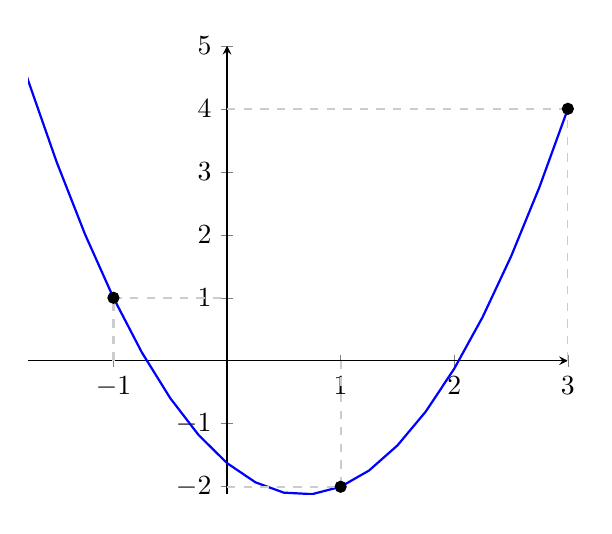
\begin{tikzpicture}
\begin{axis}[axis lines=middle,
    ymax=5, ytick distance=1]

\addplot[color=blue, thick, domain=-3:3]{(9*x^2)/8 - (3*x)/2 - 13/8};
\addplot[color=gray!40, domain=0:3, dashed, thick]{4};
\addplot[color=gray!40, domain=0:1, dashed, thick]{-2};
\addplot[color=gray!40, domain=-1:0, dashed, thick]{1};
\addplot[color=gray!40, dashed, thick]coordinates{(3,0) (3,4)};
\addplot[color=gray!40, dashed, thick]coordinates{(1,0) (1,-2)};
\addplot[color=gray!40, dashed, thick]coordinates{(-1,0) (-1,1)};
\addplot[only marks, mark=*, mark size=2pt, color=black] coordinates {(3,4)};
\addplot[only marks, mark=*, mark size=2pt, color=black] coordinates {(1,-2)};
\addplot[only marks, mark=*, mark size=2pt, color=black] coordinates {(-1,1)};

\end{axis}
\end{tikzpicture}
\end{solution}

\begin{problem}
Sketch the graph of the function \(f(x) = x^2 -3x +4\) on the interval \((-3, 5)\)
\end{problem}
\begin{solution}
lmao
\begin{tikzpicture}
\begin{axis}[axis lines = middle,
    xtick distance = 1,
    ymin=0]

\addplot[color=red, thick, domain=-3:5]{x^2 - 3*x + 4};
\addplot[only marks, mark=*, mark size=1pt, color=black] coordinates {(1.5,1.75)}
node[below] {\tiny (1.5,1.75)};

\addplot[only marks, mark=*, mark size=1pt, color=black] coordinates {(0,4)}
node[below left] {\small (0,4)};
\end{axis}
\end{tikzpicture}

The maximum value of the graph is at \(x=-3\), therefore
\[
(-3)^2 -3(-3) +4 = 9 + 9 + 4 = 22
\]
The minimum value is indicated on the graph.
\end{solution}

\begin{problem}
Draw the graph of the function \(f(x) = -2x^2 + 11x - 4\)
\end{problem}

\begin{solution}
\end{solution}
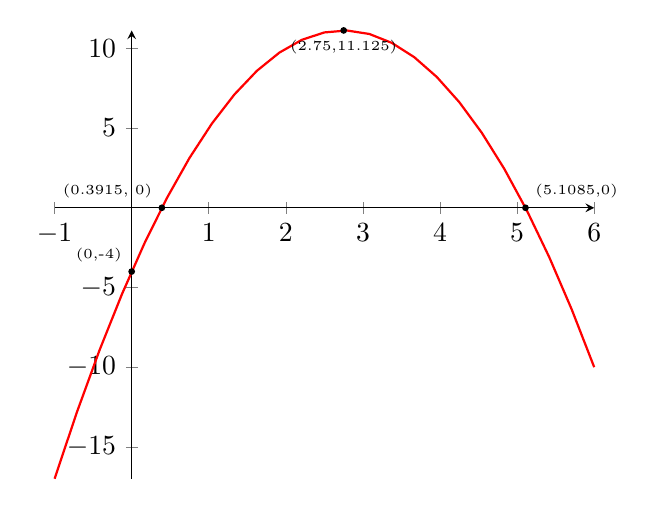
\begin{tikzpicture}
\begin{axis}[axis lines = middle, clip=false]

\addplot[color=red, thick, domain=-1:6]{-2*x^2 + 11*x - 4};
\addplot[only marks, mark=*, mark size=1pt, color=black] coordinates {(5.1085,0)}
node[above right] {\tiny (5.1085,0)};

\addplot[only marks, mark=*, mark size=1pt, color=black] coordinates {(0,-4)}
node[above left] {\tiny (0,-4)};

\addplot[only marks, mark=*, mark size=1pt, color=black] coordinates {(0.3915, 0)}
node[above left] {\tiny (0.3915, 0)};

\addplot[only marks, mark=*, mark size=1pt, color=black] coordinates {(2.75,11.125)}
node[below] {\tiny (2.75,11.125)};
\end{axis}
\end{tikzpicture}

\begin{problem}
Let \(f(x) = ax+b\) be an arbitrary linear function. Prove that \(f(f(x))\) is also linear.
\end{problem}
\begin{solution}
By definition, a linear function is one whose only power in the variable is one. No higher or lower or fractional powers are allowed. Let us compute \(f(f(x))\)
\begin{align*}
f(f(x)) &= f(ax+b) \\
    &=a(ax+b) + b\\
    &=a^2x + ab + b \\
    &=a'x + b' &&\because let\ a^2 = a', \ ab+b =b'
\end{align*}
Note that we can perform the last step since \(a\) and \(b\) are constants.
The power of \(x\) is still one in the final expression. Therefore the composition of two linear functions is linear. 
\end{solution}

\begin{problem}
For the following functions
\begin{align*}
f(z) &= \sqrt{4-z^2} \\
g(x) &= 2x +3
\end{align*}
Find the domain of \(y = f(g(x))\) for which \(y\) is well defined.
\end{problem}
\begin{solution}
We first immediately note that both the domain and range of \(g(x)\) are the entirety of \(\mathbb{R}\). The only restriction then comes from \(f(z)\). To find the domain of \(f(z)\) we must find the interval for which the square root is non-negative
\begin{align*}
4-z^2 &\geq 0 \\
z^2  &\leq 4 \\
z &\leq |2|
\end{align*}
Now that we know the domain of \(f(z)\), we now have to find the interval such that \(-2 \leq g(x) \leq 2\). Since \(g\) is a monotone function and nicely invertible, we can find the inverse of \(g\) and plug in the values 2 and -2 to obtain the interval for our required domain.
\begin{align*}
g(x) &= 2x +3 \\
g^{-1}(x) &= \frac{x-3}{2} \\
g^{-1}(-2) &= \frac{-2 -3}{2} &= \frac{-5}{2} \\
g^{-1}(2) &= \frac{2 -3}{2} &= \frac{-1}{2}
\end{align*}
Thus the domain of our function \(y = f(g(x))\) is \(\left[-\frac{5}{2},\frac{-1}{2}\right]\)

\begin{problem}
Find the inverse of \(f(x) = \sqrt{x} + \sqrt{x-1}\) and its applicable domain.
\end{problem}
\begin{solution}
By observation we see that \(f(x)\) has a domain \([1, \infty)\). Since it is a monotone increasing function we can find its range via plugging in the endpoints of the domain
\begin{align*}
f(1) &= \sqrt{1} + \sqrt{1-1} = \sqrt{1} \\
\lim_{x\to \infty} f(x)&= \lim_{x\to \infty} \sqrt{x} + \lim_{x\to \infty} \sqrt{x-1} = \infty
\end{align*}
\end{solution}
Therefore our range is \([1, \infty)\) as well and this will be the domain of our inverse function. To find the inverse function itself we must do some rather annoying algebraic manipulation
\begin{align*}
y &= \sqrt{x} + \sqrt{x-1} \\
y^2 &= x + x-1 + 2(\sqrt{x})(\sqrt{x-1}) \\
y^2 -2x +1 &= 2\sqrt{x}\sqrt{x-1} \\
y^4 -4y^2x +2y^2 +4x^2 -4x +1 &= 4x^2-4x \\
y^4 -4y^2x +2y^2 +1 &= 0 \\
x &= \frac{y^4 +2y^2 +1}{4y^2} \\
x &= \left(\frac{y^2+1}{2y}\right)^2
\end{align*}
\end{solution}

\begin{problem}
Find the solution for \(\frac{x+1}{x-2} \leq \frac{x+2}{x+3}\).
\end{problem}
\begin{solution}
\begin{align*}
\frac{x+1}{x-2} - \frac{x+2}{x+3} &\leq 0 \\
\frac{(x+1)(x+3) - (x+2)(x-2)}{(x-2)(x+3)} &\leq 0 \\
\frac{x^2 +4x + 3 - x^2 + 4}{(x-2)(x+3)} &\leq 0 \\
\frac{4x + 7}{(x-2)(x+3)} &\leq 0 \\
\end{align*}

The domain splits of the above function are \((-\infty, -3),\ (-3, -1.75),\ (-1.75, 2),\ (2, \infty)\). We can again use a table to find out the final signature results of our function

\[
\begin{array}{c|c|c|c|c}
Interval & 4x+7 & x-2 & x+3 & Sign \\
\midrule
(-\infty, -3) & - & - & - & - \\
(-3, -1.75) & - & - & + & + \\
(-1.75, 2) & + & - & + & - \\
(2, \infty) & + & + & + & + \\
\end{array}
\]

Therefore our solution set is \((-\infty, -3) \cup (-1.75, 2)\)
\end{solution}

\begin{problem}
Find the solution of \(\frac{3x}{x^2+2} \geq \frac{1}{x-1}\)
\end{problem}
\begin{solution}
\begin{align*}
\frac{3x}{x^2+2} - \frac{1}{x-1} &\geq 0 \\
\frac{3x(x-1) - (x^2+2)}{(x^2+2)(x-1)} &\geq 0 \\
\frac{2x^2 -3x -2}{(x^2+2)(x-1)} &\geq 0 \\
\frac{(2x+1)(x-2)}{(x^2+2)(x-1)} &\geq 0 \\
\end{align*}
Since \(x^2+2\) is always positive, we don't need to split the domain with respect to that term, for the rest we obtain \(\left(-\infty, -\frac{1}{2}\right),\ \left(-\frac{1}{2}, 1\right),\ (1, 2),\ (2, \infty)\). The table looks like

\[
\begin{array}{c|c|c|c|c}
Interval & 2x+1 & x-2 & x-1 & Sign \\
\midrule
\left(-\infty, -\frac{1}{2}\right) & - & - & - & - \\
\left(-\frac{1}{2}, 1\right) & + & - & - & + \\
(1, 2) & + & - & + & - \\
(2, \infty) & + & + & + & + 
\end{array}
\]

For positivity, our required intervals are \(\left(-\frac{1}{2}, 1\right) \cup (2, \infty)\)
\end{solution}


\end{document}
